%\documentclass[a4paper,english,11pt,twoside]{article}
\documentclass[a4paper,english,11pt]{article}

\usepackage[utf8]{inputenc}
\usepackage[T1]{fontenc, url}
\usepackage[english]{babel}
%\usepackage{epsfig}
\usepackage{graphicx}
\usepackage{amsmath}
\usepackage{mathtools}
\usepackage{pstricks}
\usepackage{subfig}
\usepackage{epstopdf}
\usepackage{varioref}
\usepackage{listings}
\usepackage{xcolor}
\usepackage{float}
\usepackage[]{mcode}
\usepackage{verbatim}
\usepackage{gensymb}
\usepackage{caption}

\lstset{ 
  captionpos=b,
  frame=tb,
  numbers=left}
\urlstyle{sf}
\usepackage[margin=1 in]{geometry} % Setter margene til word standard

\usepackage{ifikompendiumforside}


\newcommand{\tab}[1]{\hspace{.2\textwidth}\rlap{#1}}

\newcommand{\itab}[1]{\hspace{0em}\rlap{#1}}

%%%%%%%%%%%%%%%%%% END HEADER

\title{Laboratory Assignment 3}
\subtitle{INF4411\\ 
          Analog Microelectronics}

\author{
\begin{tabular}{ r c l }
  Rikesh Chauhan & & rikesh.chauhan@fys.uio.no\\
  Espen Klein Nilsen & & e.a.k.nilsen@fys.uio.no\\
  Vegard Midtbøen & & vegard.midtboen@fys.uio.no
\end{tabular}
}
%{Rikesh Chauhan rikesh.chauhan@fys.uio.no\\
%	Espen Klein Nilsen e.a.k.nilsen@fys.uio.no\\
%	Vegard Midtbøen vegard.midtboen@fys.uio.no} 

\begin{document}
\ififorside

\tableofcontents

\newpage
%//////////////////////////////////////Task1///////////////////////////////////////////////////////////////////////        
\section{Task 1}
The circuit shown in Figure \ref{fig:chem} shows the chematic drawn in Cadence for the given curcuit.
\begin{figure}[!htbp]
 \centering
  \fbox{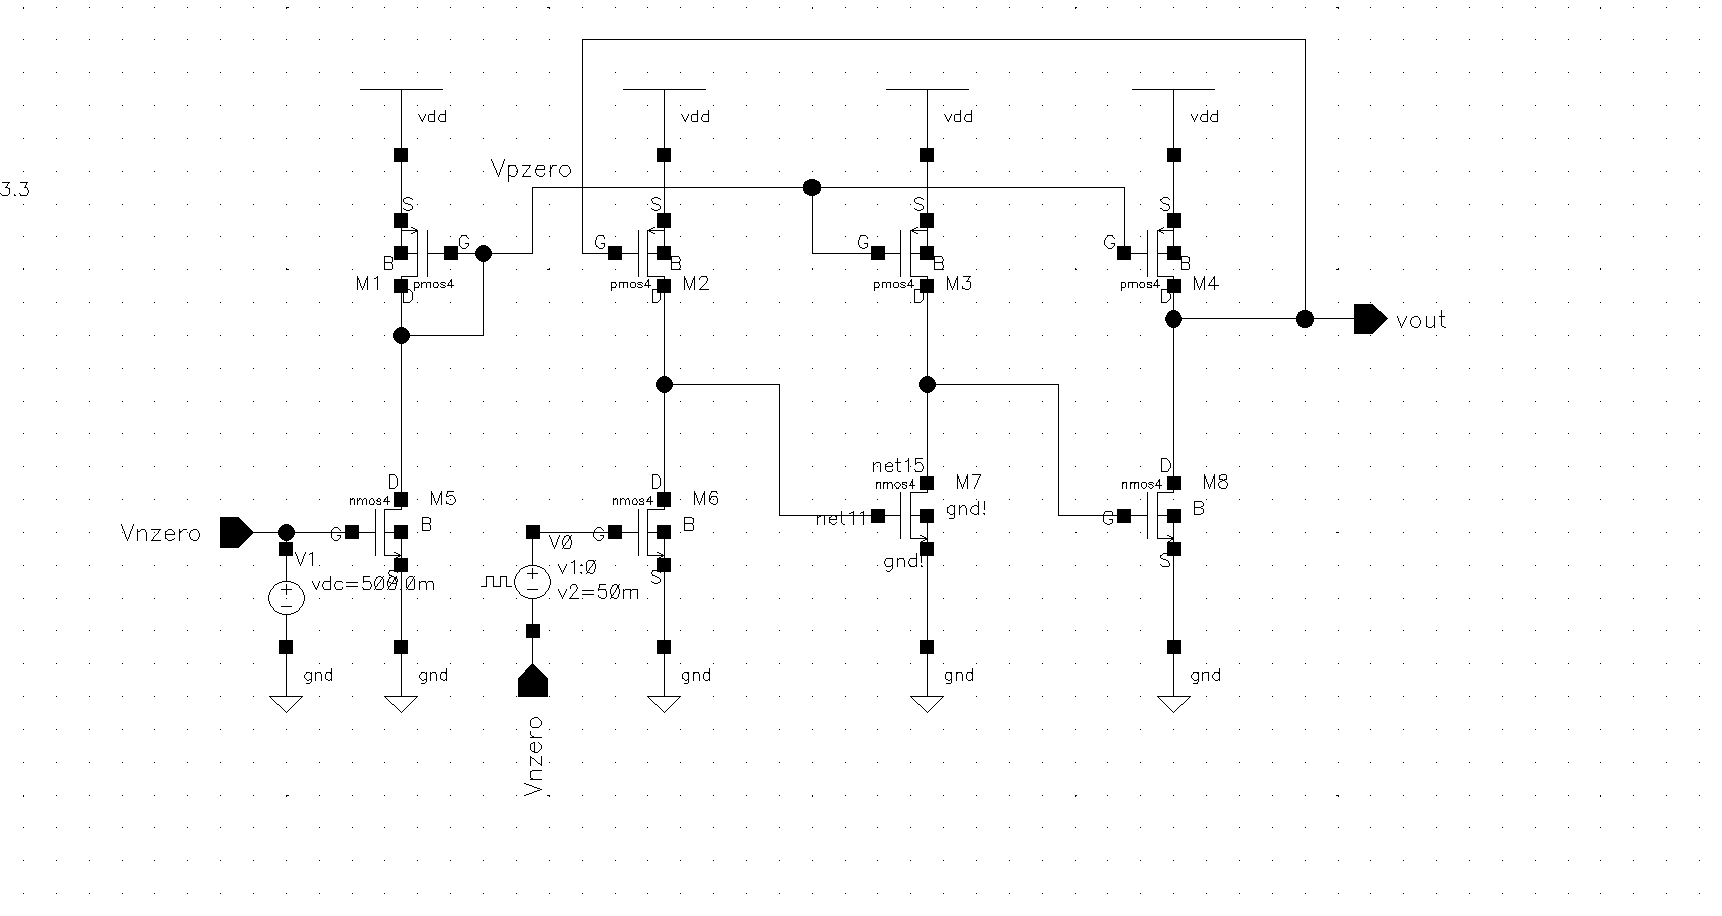
\includegraphics[width=\textwidth]{img/chematic_bi-color}}
  \caption{Chematic drawing from Cadence.}
  \label{fig:chem}	
\end{figure}


\section{Task 2}
\textbf{1.1}\\
The simulation parameters we used for this simulation is listed below:\\
\begin{enumerate}
  \item \itab{$V_{DD}$:} \tab{3.3 V}
  \item \itab{$V_{nzero}$:} \tab{500 mV} \tab{(DC-Offset)}
  \item \itab{$V_{step}$:} 
  \begin{enumerate}
    \item \itab{$Amplitude$:} \tab{$50 mV$}
    \item \itab{$Rise time$:} \tab{$100 ns$}
  \end{enumerate}
  \item \itab{W/L} \tab{$10\mu m/0.35\mu m$}  
  \item \itab{$V_{sweep}$} \tab{0 - 6 V}
\end{enumerate}
A plot of the output and input for the circuit is shown in Figure \ref{fig:sim:ring}. From the plot we can se that 
after a \textit{steep} step we get oscillations on the output that reaches $Vdd$. The peak to peak voltage is $1.2 V$.
The simulation is so resource intencive that we were forced to only run the simulation for a short time (or shorter 
than the task spesified).\\

\begin{figure}[!htbp]
 \centering
  \fbox{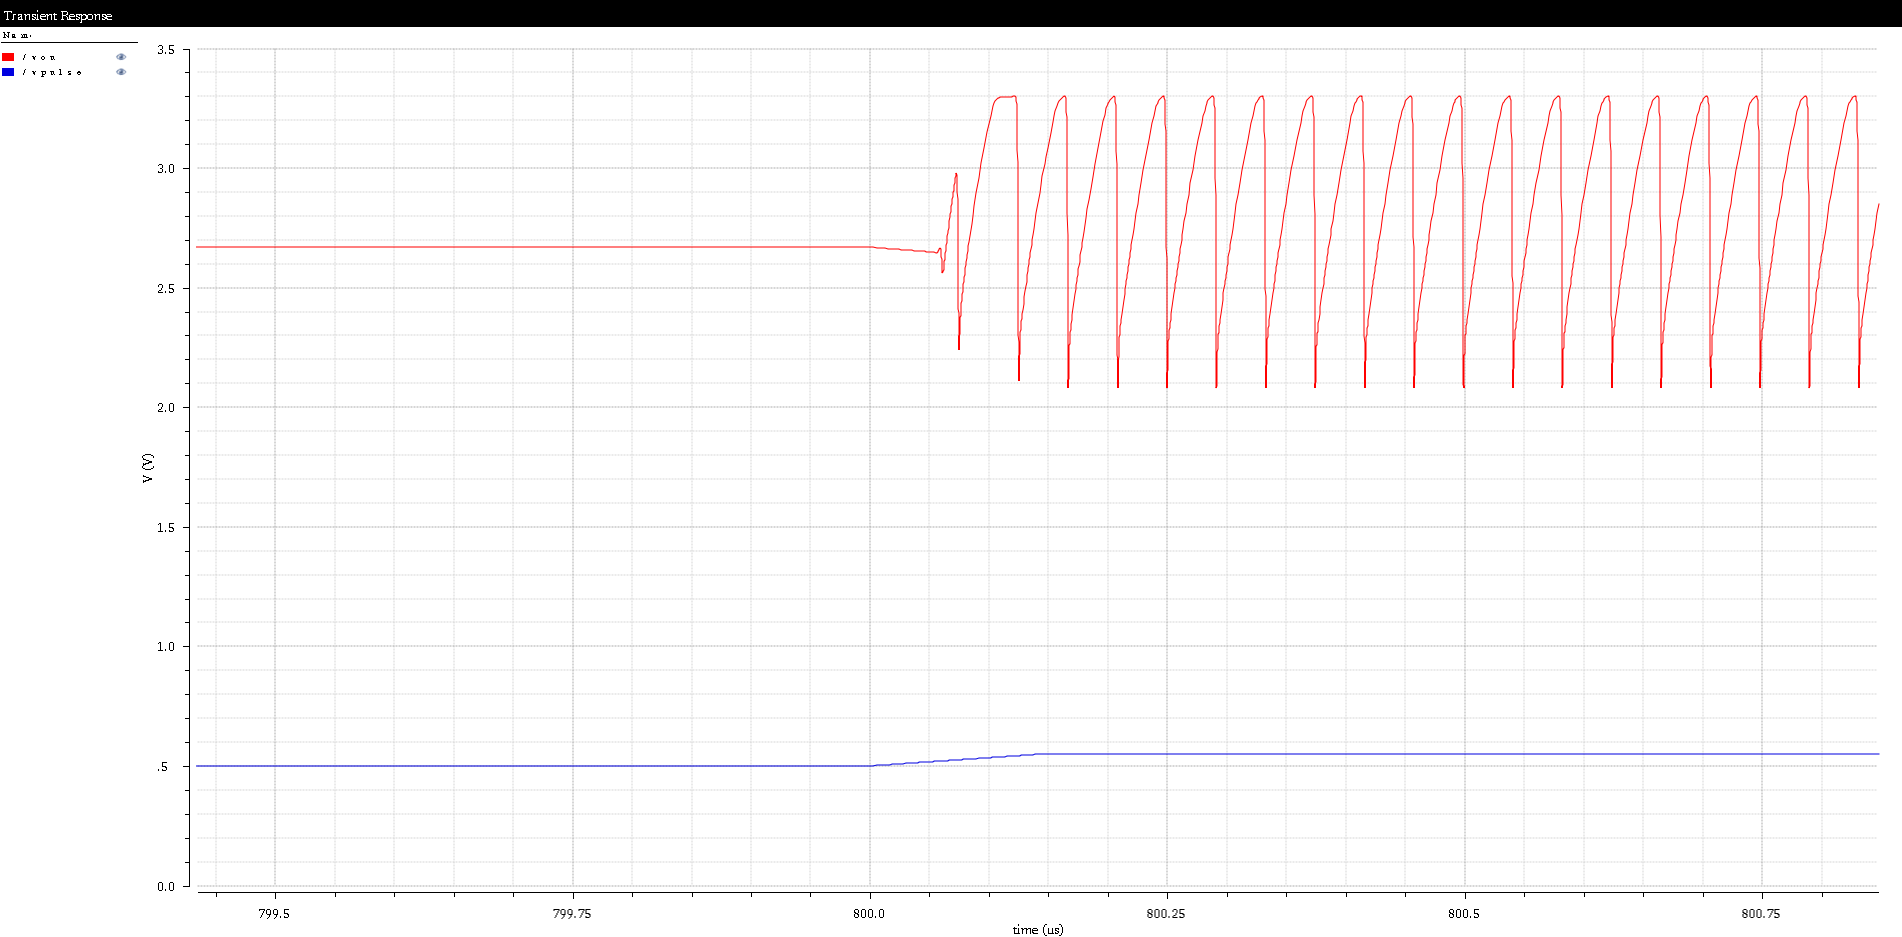
\includegraphics[width=\textwidth]{img/simulation_with_ringing}}
  \caption{Simulation with ringing.}
  \label{fig:sim:ring}	
\end{figure}
\newpage
\textbf{1.2}\\
The AC responce is plottet in Figure \ref{fig:ac:responce}\\
\begin{figure}[!htbp]
 \centering
  \fbox{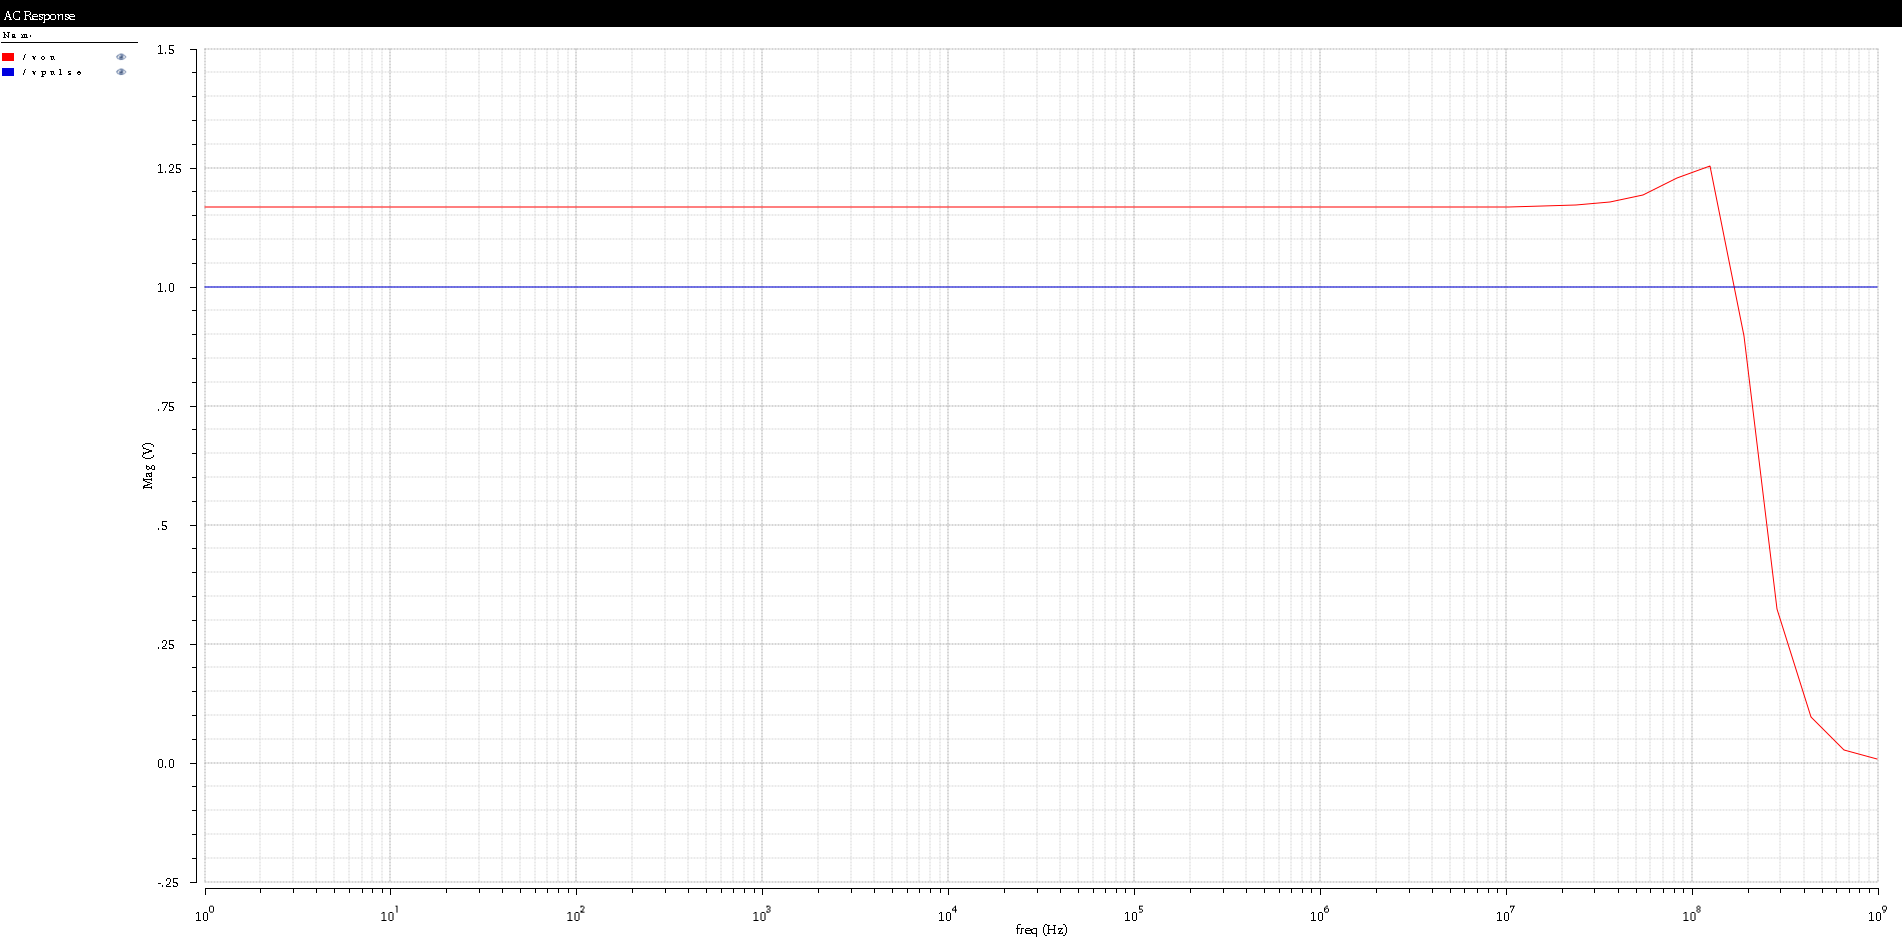
\includegraphics[width=\textwidth]{img/ac_responce}}
  \caption{Plot of AC responce.}
  \label{fig:ac:responce}	
\end{figure}

The frequency of the oscillations is about 24 MHz in the cadence simulation. There is a maximum at 120MHz in the AC-simulation. The   resonance appears to start at 24MHz, witch could give rise to the ringing on the output. 

\section{Task 3}
In order to find the value of $C_{c1}$ which corresponds to different phase margins, we looked table 5.1 of the text books and found that$ 20\degree$, $40\degree$ and $60\degree$  phase margin is equal to 56.95\%, 28.93\% and 8.77\% overshoot. So we ran transient simulation with varying  $C_{c1}$ to get these overshoot.\\

Figure \ref{pm20} is the overshoot plot that we got for  $C_{c1} = 1.13 nF$ where overshoot is 56.95\%. This corresponds to the phase margin of $20\degree$
\begin{figure}[H]
 \centering
  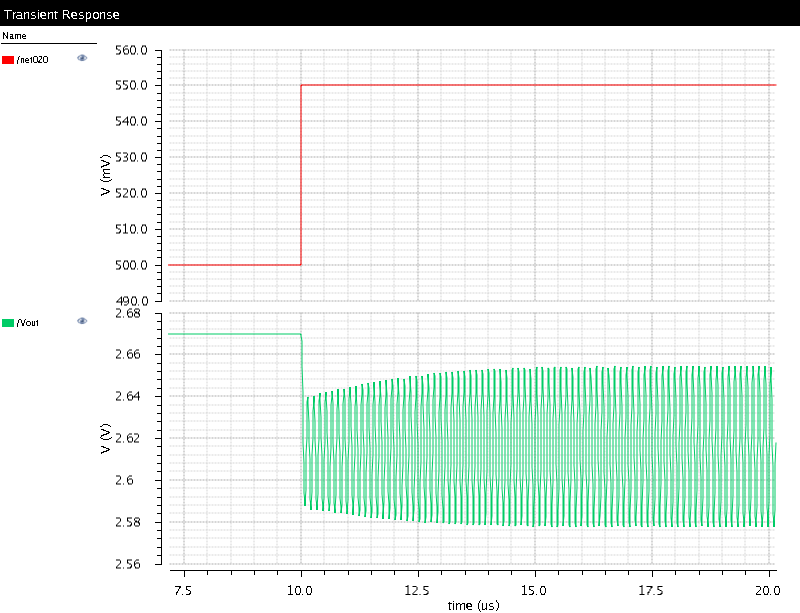
\includegraphics[width=0.8\textwidth]{img/cad_pm/pm_20_1_13nF.png}
  \caption{56.95\% overshoot for $C_{c1} = 1.13nF$}
  \label{pm20}	
\end{figure}

Figure \ref{pm40} is the overshoot plot that we got for  $C_{c1} = 1.35 nF$ where overshoot is 28.93\%. This corresponds to the phase margin of $40\degree$
\begin{figure}[H]
 \centering
  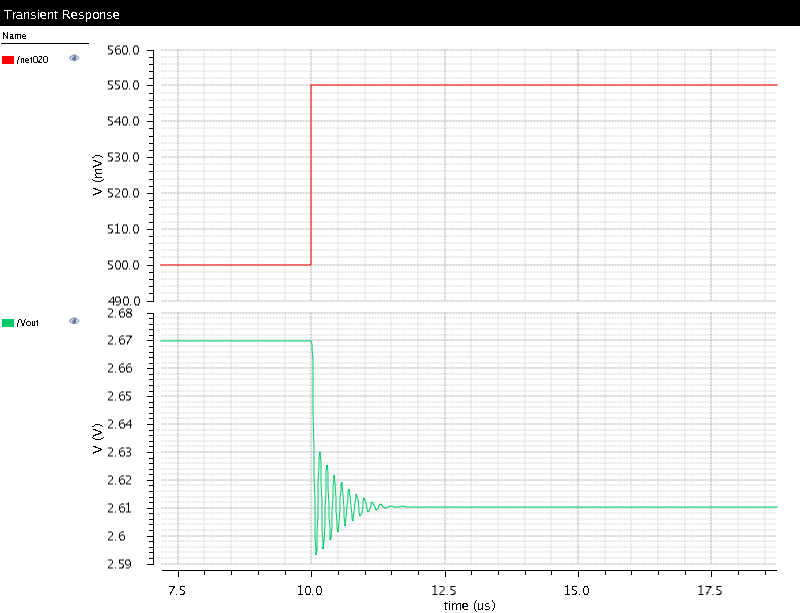
\includegraphics[width=0.8\textwidth]{img/cad_pm/pm_40_1_35nF.png}
  \caption{28.93\% overshoot for $C_{c1} = 1.35nF$}
  \label{pm40}	
\end{figure}

Figure \ref{pm60} is the overshoot plot that we got for  $C_{c1} = 2 nF$ where overshoot is 8.77\%. This corresponds to the phase margin of $60\degree$
\begin{figure}[H]
 \centering
  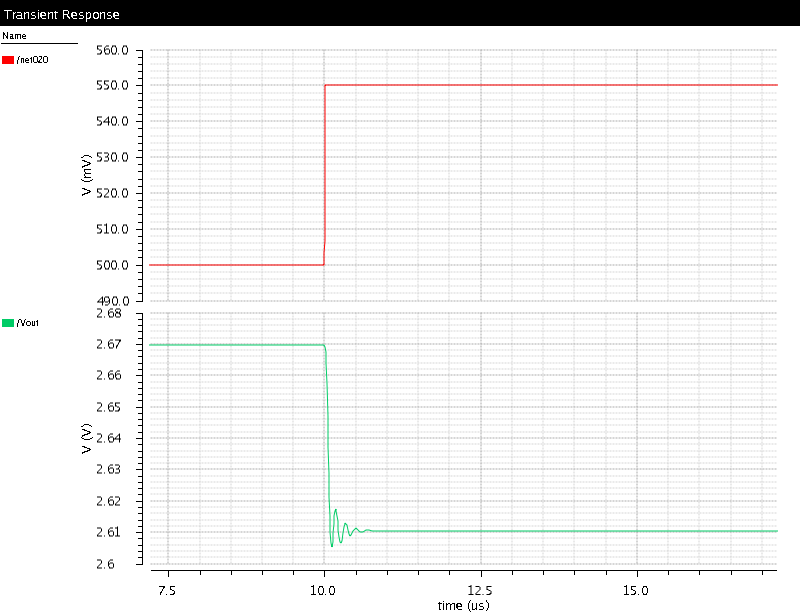
\includegraphics[width=0.8\textwidth]{img/cad_pm/pm_60_2nF.png}
  \caption{8.77\% overshoot for $C_{c1} = 2nF$}
  \label{pm60}	
\end{figure}


\section{Task 4}

\section{Task 5}
Figure \ref{fig:pcb} shows the PCB for this task. We decided to make a new PCB because the awailable transistor in the lab, was not the same as in the previos labs.
\begin{figure}[!htbp]
 \centering
  \fbox{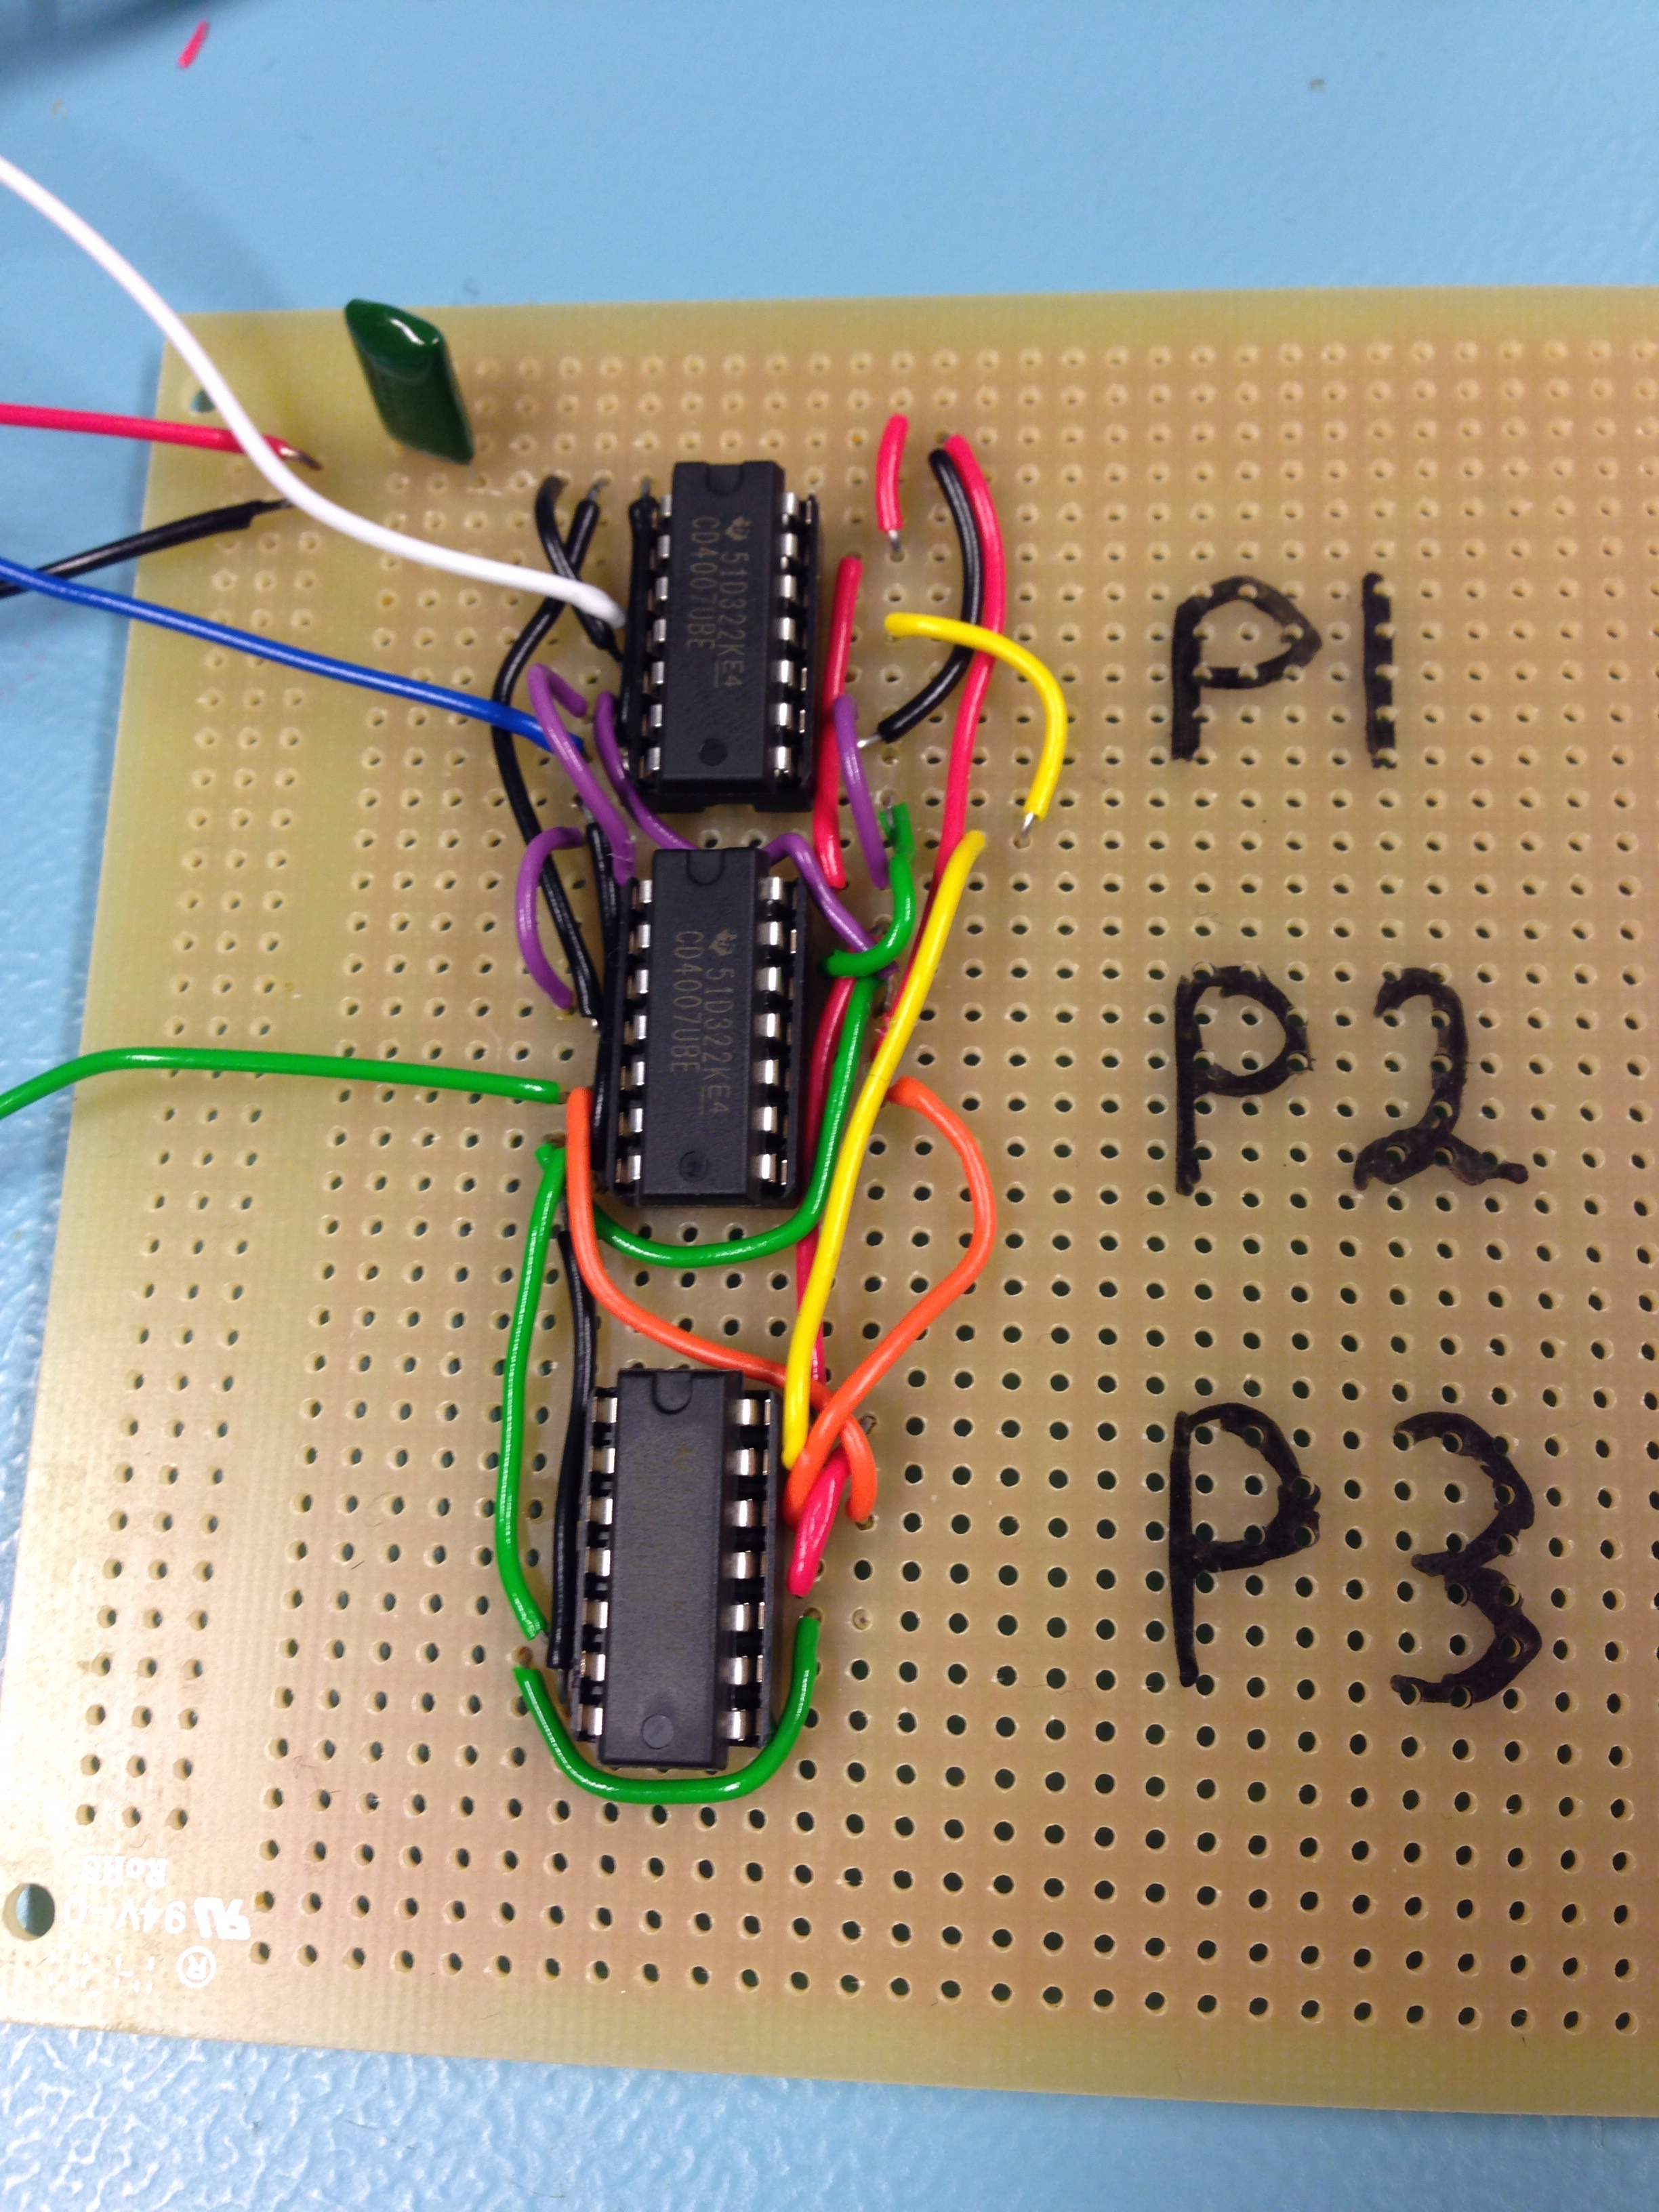
\includegraphics[width=0.8\textwidth]{img/pcb}}
  \caption{PCB for task 5.}
  \label{fig:pcb}	
\end{figure}
In the task, it was given that $V_{DD}$ was suppose to be $10 V$. For $V_{DD}$ we used the voltage source available in the lab, and used the $+ 25V$ port.
The voltage for $V_{nzero}$ was also provided from the voltage source, using the $+ 6V$ port.\\
\\
To find a proper $V_{nzero}$, we connencted the oscilloscope to the output. By doing this, we could determine which value for $V_{nzero}$ that gave the 
most symetrical outout. We found this bias voltage to be $3.8V$. When this was set, we made a simple matlab script (see appendix X), controlling the 
voltage supply and the oscilloscope. The plot for the output can be seen in Figure \ref{fig:oscil:out}.\\
\\
The circuit is not stable. What we see from the plot in Figure \ref{fig:oscil:out} is oscillation/ringing. The frequency for the oscillation is
$5.348 MHz$.
\begin{figure}[!htbp]
 \centering
  \fbox{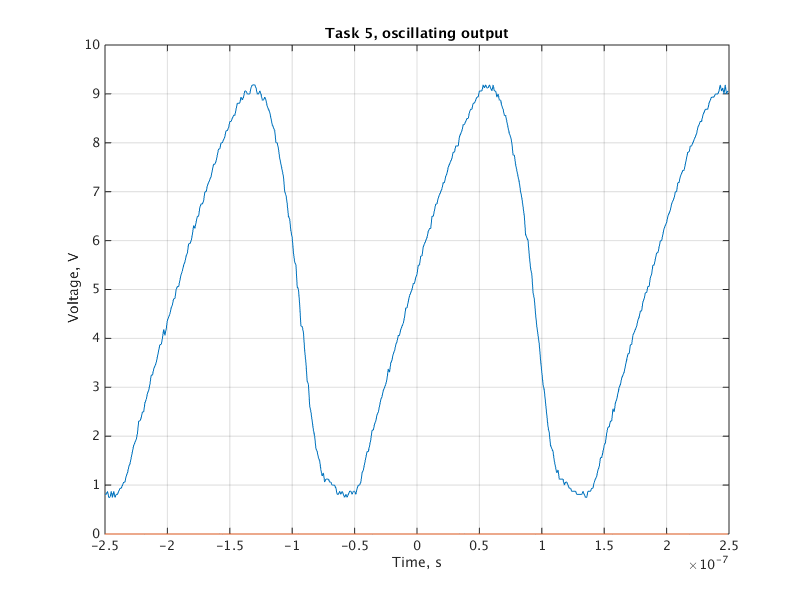
\includegraphics[width=\textwidth]{img/task5_oscillating_output}}
  \caption{Oscillating output at Vdd/2.}
  \label{fig:oscil:out}	
\end{figure}

\section{Task 6}
In this task, we have cutted the feedback loop. Since voltage sources are limited in the lab, we soldered a potensiometer to the PCB
in order to make a proper $V_{nzero}$. The task is saying that we need to separate the two inputs for $V_{nzero}$, and create a proper $V_{pzero}$.
Instead of breaking the circuit at the point where $V_{pzero}$ is labeled in the lab descrition, we applied different voltages for the two 
$V_{nzero}$ points, and found a proper $V_{pzero}$ by meauring the point. We found it best to sweep the $V_{nzero}$ point, and keeping the $V_{pzero}$ constant.
\\
\\
The linear line segment in the plot, is the an average plot of the oscillatios. As the bias voltage change the duty cycle of the osccilations change, moving the 
avraged DC value measured. The frequency of the oscillations is about 135 MHz. 
The estimated line (shown in red, Figure \ref{fig:mes:approx:gain}) is probably a more acurate depiction of the gain.
(This can be seen if we compare the two points in figures \ref{fig:vnzero:vout} and \ref{fig:scope:plot:lin}.)\\
\\
From the measurment we calculate the gain to be \underline{-99,3226}.\\
\\
Points:\\
P1 = (3,926 , 9,973)\\
P2 = (4,019 , 0,736)\\
\\
Equation:
\begin{center}
$m = (Y2 - Y1) / (X2 - X1)$\\
$Y = m(X - X1) + Y1$\\
$Y = -99,3 * (X - 3,926) + 9,973$
\end{center}
We can se from the plot in Figure \ref{fig:mes:approx:gain}, that the gain in the area ~ 4.018 - 4.019, the gain is very large, and it is almost imposible to find a propper
point for calculating the gain. We were not able to get the exact point of operation do to oscillations at the output. 

\begin{figure}[!htbp]
 \centering
  \fbox{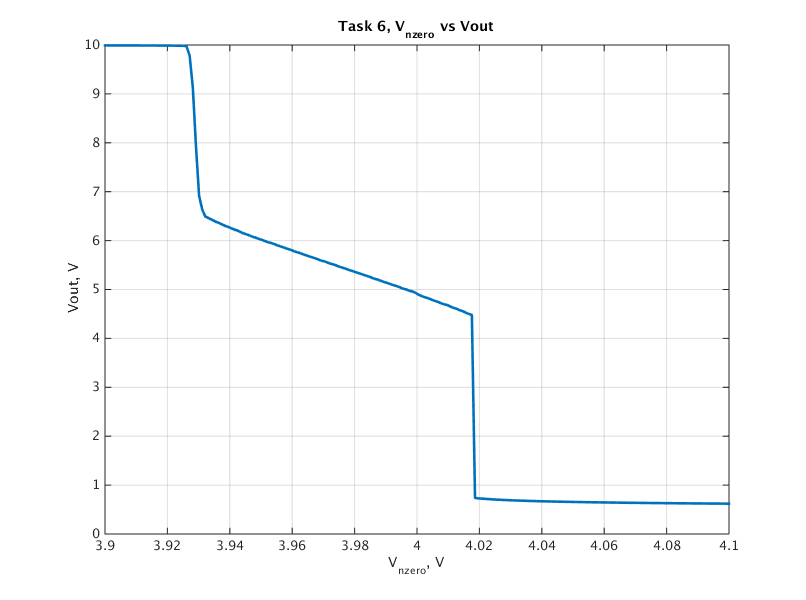
\includegraphics[width=0.8\textwidth]{img/task6_vnbias_vs_vout}}
  \caption{Plot og $V_{nzero}$ vs Vout.}
  \label{fig:vnzero:vout}	
\end{figure}

\begin{figure}[!htbp]
 \centering
  \fbox{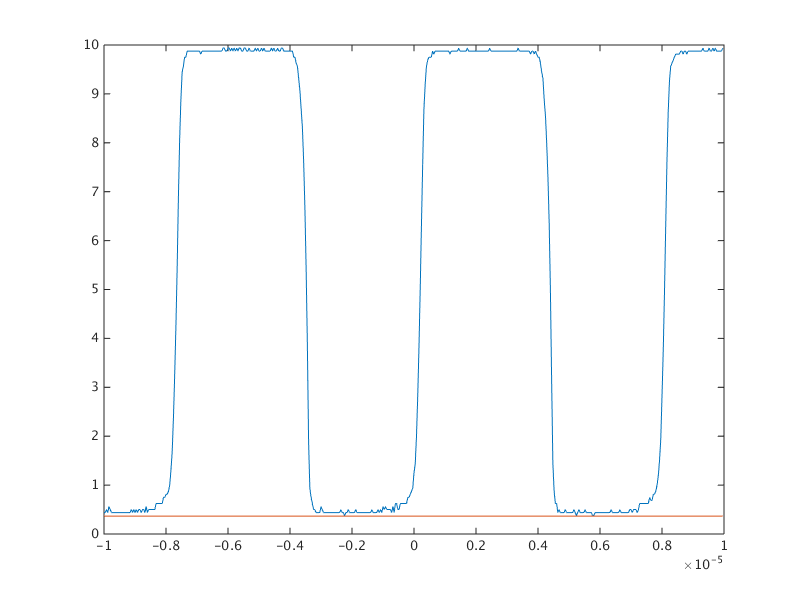
\includegraphics[width=0.8\textwidth]{img/task6_scope_plot_lin_area}}
  \caption{Plot from oscilloscope for the linear area.}
  \label{fig:scope:plot:lin}	
\end{figure}
\begin{figure}[!htbp]
 \centering
  \fbox{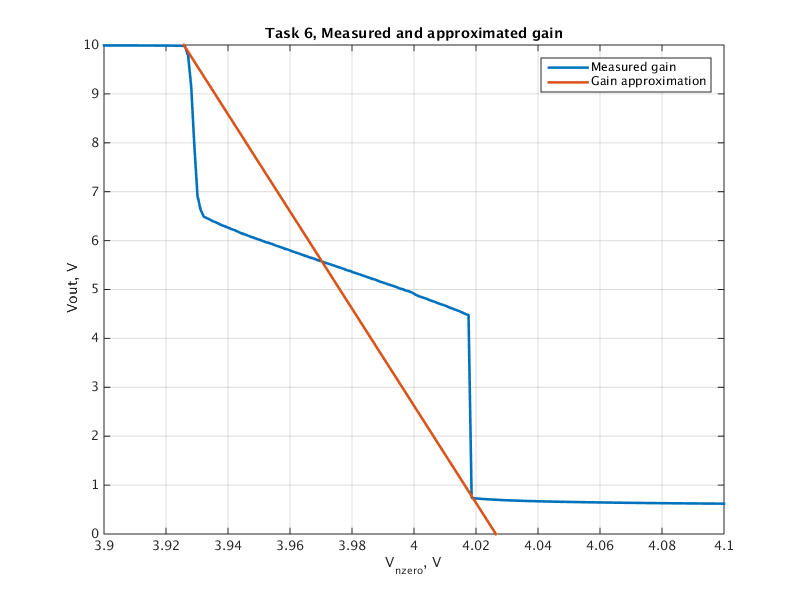
\includegraphics[width=0.8\textwidth]{img/task6_measured_and_approximated_gain}}
  \caption{Measured and approximated gain.}
  \label{fig:mes:approx:gain}	
\end{figure}

%\begin{figure}[htbp]
% \centering
%  \fbox{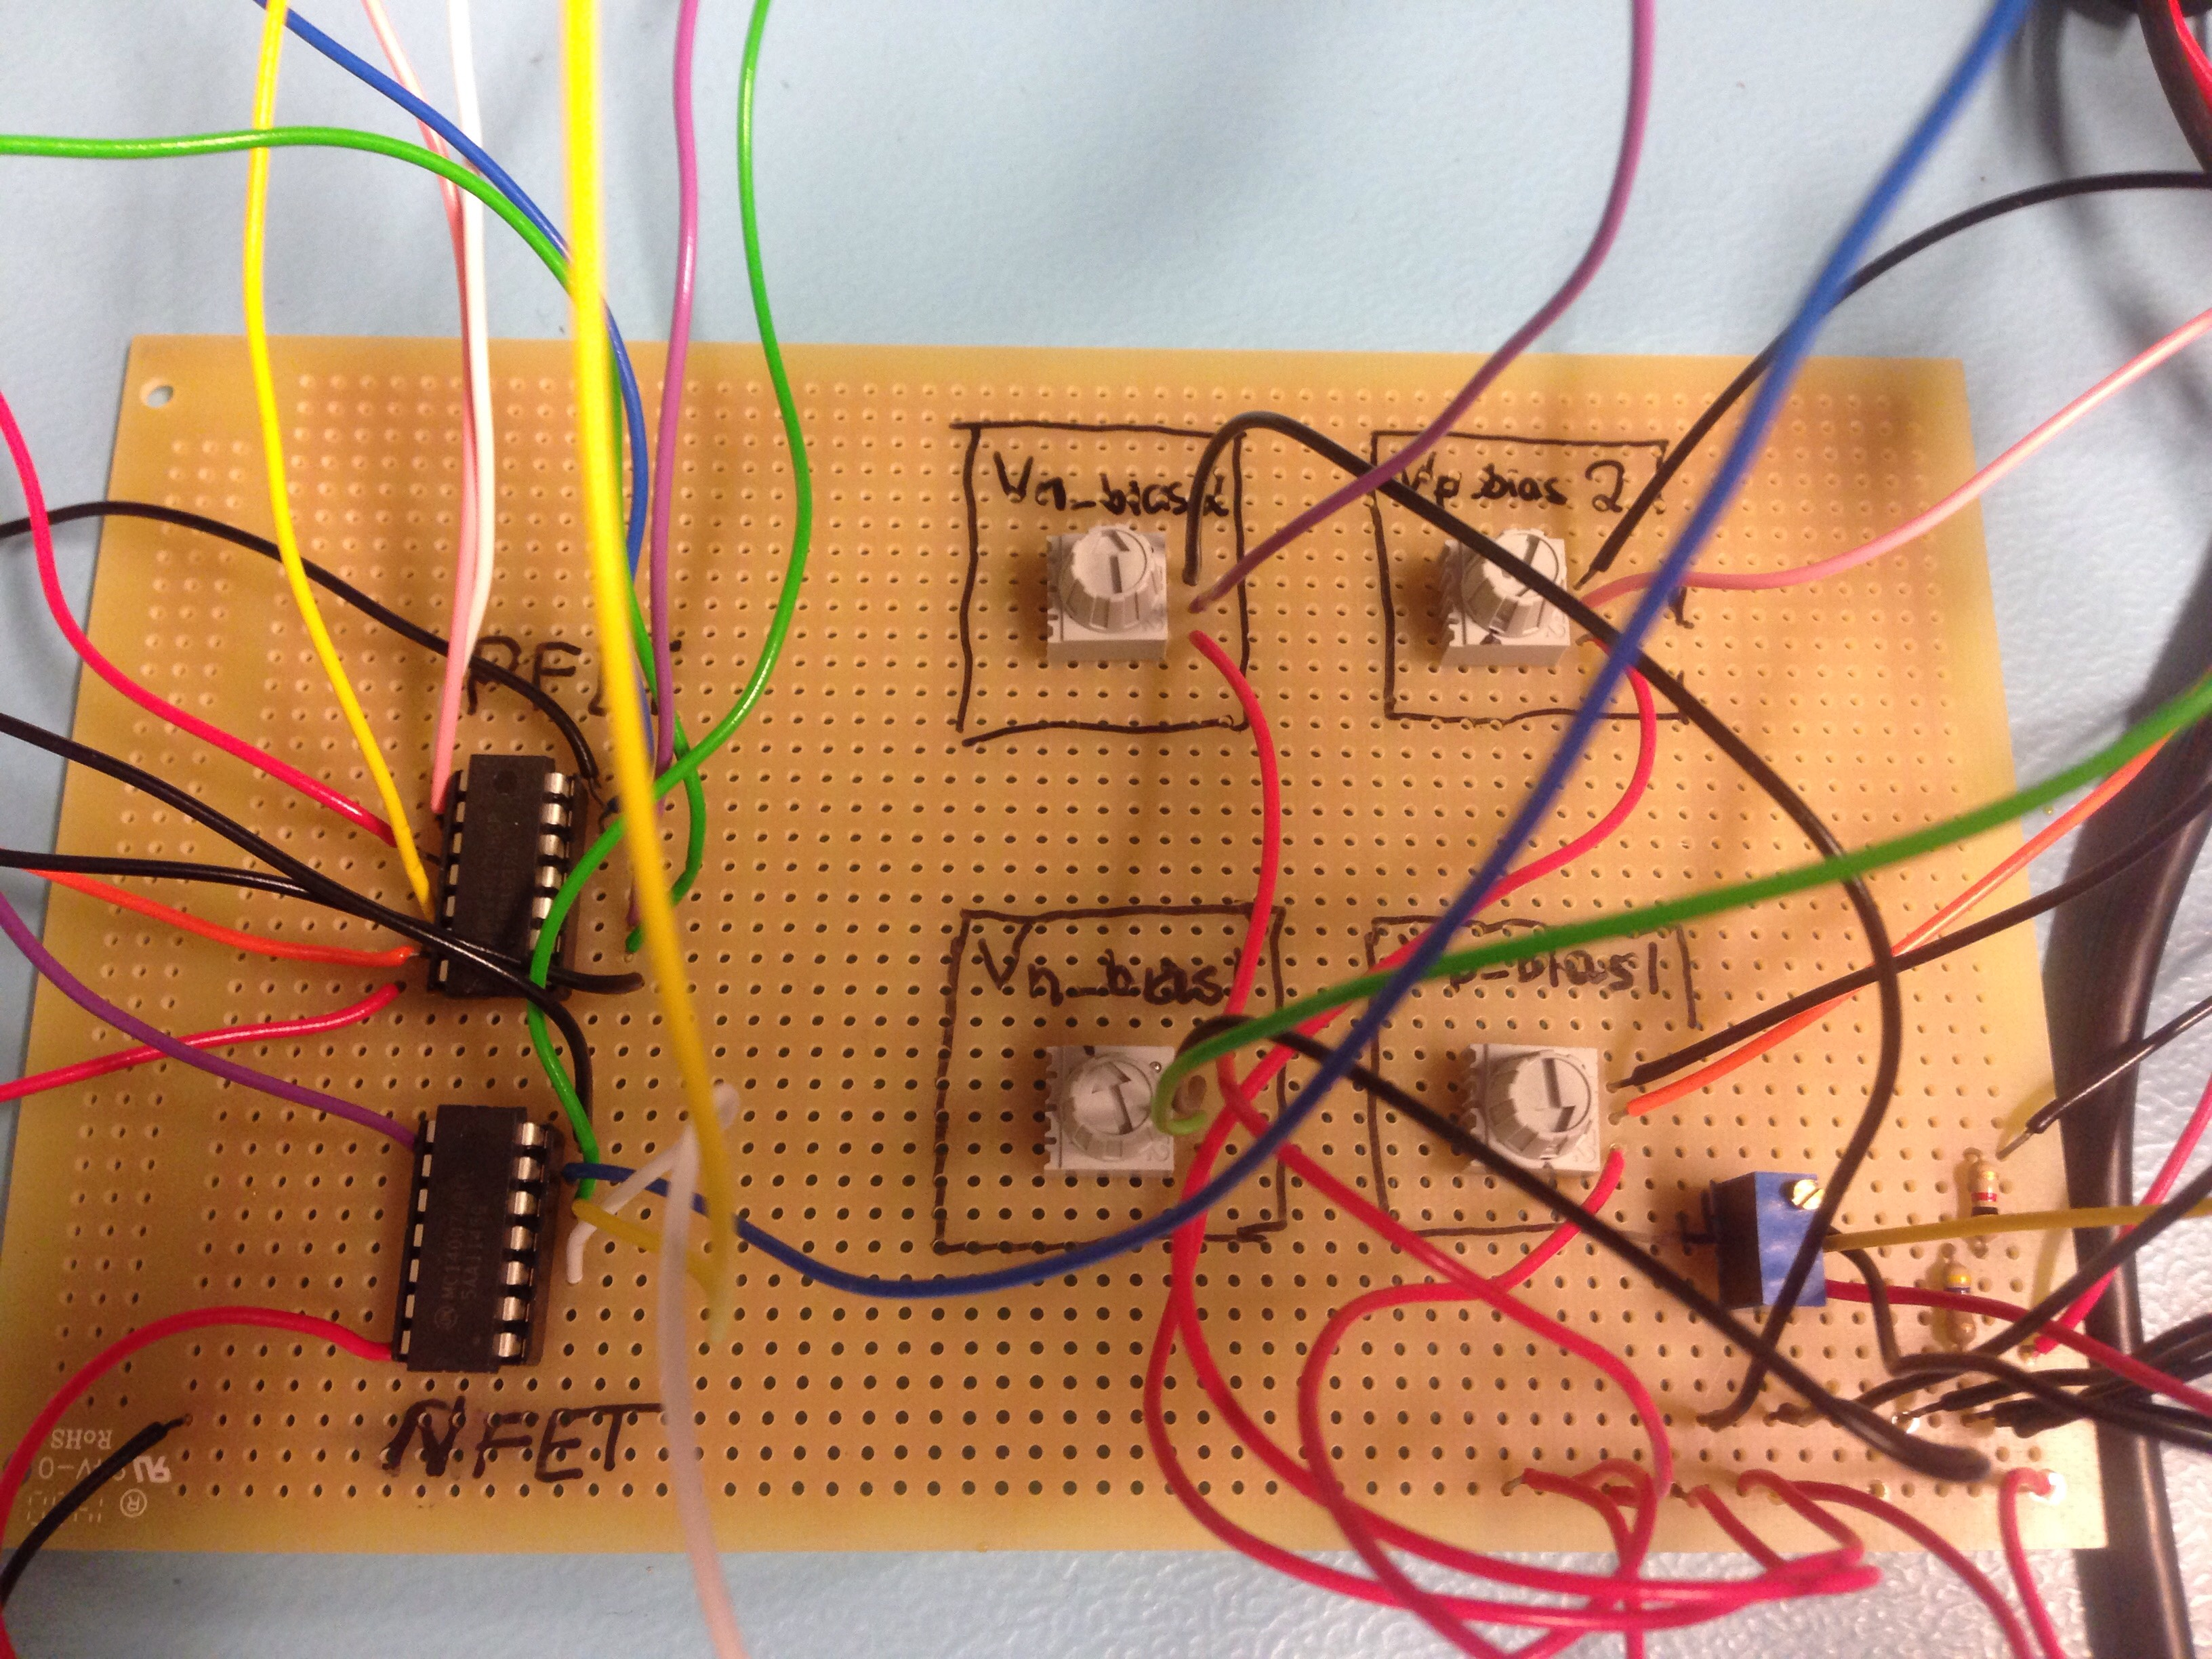
\includegraphics[width=\textwidth]{img/pcb_setup}}
%  \caption{Final PCB board.}
%  \label{fig:pcb}	
%s\end{figure}



\end{document}
